\documentclass[a4paper,12pt,twoside]{report} % TODO: add `openright` option when you have at least 50 pages

% Packages
\usepackage{amsmath} % -> Matrices, `pmatrix` command
\usepackage{auto-pst-pdf} % -> Dependency of psfrag. Add `-shell-escape` paramter to pdflatex command in Commands menu
\usepackage[top=2cm, bottom=2.5cm, inner=2cm, outer=2cm, bindingoffset=1.5cm]{geometry} % -> Makes custom margins for the twoside document style. Use `\usepackage{showframe}` command to show the margins
\usepackage{graphicx} % -> Images, `includegraphics` command
\usepackage[parfill]{parskip} % -> Makes new paragraphs without indentation.
\usepackage{psfrag} % -> To be able to change text font on matlab exports, `psfrag` command

% Other configuration
\graphicspath{{./Resources/}}
% Replace these texts on .eps pictures
\psfrag{t[s]}{$t$[s]}
\psfrag{x[m]}{$x$[m]}
\psfrag{h[m]}{$h$[m]}
\psfrag{v[km/h]}{$v$[km/h]}
\psfrag{v[m/s]}{$v$[m/s]}
\psfrag{vstac[km/h]}{$v_{\rm stac}$[km/h]}
\psfrag{hstac[m]}{$h_{\rm stac}$[m]}

\psfrag{h2-1}{\tiny $h_{\rm 21}$}
\psfrag{h3-2}{\tiny $h_{\rm 32}$}
\psfrag{h4-3}{\tiny $h_{\rm 43}$}
\psfrag{h5-4}{\tiny $h_{\rm 54}$}

\psfrag{h1}{\tiny $h_{\rm 1}$}
\psfrag{h2}{\tiny $h_{\rm 2}$}
\psfrag{h3}{\tiny $h_{\rm 3}$}
\psfrag{h4}{\tiny $h_{\rm 4}$}
\psfrag{h5}{\tiny $h_{\rm 5}$}
\psfrag{h6}{\tiny $h_{\rm 6}$}
\psfrag{h7}{\tiny $h_{\rm 7}$}
\psfrag{h8}{\tiny $h_{\rm 8}$}
\psfrag{h9}{\tiny $h_{\rm 9}$}
\psfrag{h10}{\tiny $h_{\rm 10}$}

\psfrag{v1}{\tiny $v_{\rm 1}$}
\psfrag{v2}{\tiny $v_{\rm 2}$}
\psfrag{v3}{\tiny $v_{\rm 3}$}
\psfrag{v4}{\tiny $v_{\rm 4}$}
\psfrag{v5}{\tiny $v_{\rm 5}$}
\psfrag{v6}{\tiny $v_{\rm 6}$}
\psfrag{v7}{\tiny $v_{\rm 7}$}
\psfrag{v8}{\tiny $v_{\rm 8}$}
\psfrag{v9}{\tiny $v_{\rm 9}$}
\psfrag{v10}{\tiny $v_{\rm 10}$}

\psfrag{carcount}{$n [-]$}

\psfrag{l1}{\tiny $l_1$}
\psfrag{l2}{\tiny $l_2$}

\psfrag{Lane#1}{Lane 1}
\psfrag{Lane#2}{Lane 2}

\psfrag{dt=    0.4}{\scriptsize $\Delta t=0.4$}
\psfrag{dt=    0.2}{\scriptsize $\Delta t=0.2$}
\psfrag{dt=    0.1}{\scriptsize $\Delta t=0.1$}
\psfrag{dt=   0.05}{\scriptsize $\Delta t=0.05$}
\psfrag{dt=  0.025}{\scriptsize $\Delta t=0.025$}
\psfrag{dt= 0.0125}{\scriptsize $\Delta t=0.0125$}
\psfrag{dt=0.00625}{\scriptsize $\Delta t=0.00625$}

\psfrag{relativehibap[\%]}{Relative error [\%]}
\psfrag{relativehibav[\%]}{Relative error [\%]}
\psfrag{SelfDrivingCarCount}{\qquad\;$n_a$ [-]}
\psfrag{dt[s]}{$\Delta$t[s]}

% Custom commands
\newcommand{\amax}{a_{\rm max}}
\newcommand{\bmax}{b_{\rm max}}
\newcommand{\vd}{ {v_{\rm d}}}
\newcommand{\afree}{a_{\rm free}}
\newcommand{\vt}{v(t)}
\newcommand{\afollower}{a_{\rm follower}}
\newcommand{\hd}{h_{\rm d}(t)}
\newcommand{\h}{h(t)}
\newcommand{\posleader}{x_{\rm lead}(t)}
\newcommand{\lengthleader}{L_{\rm lead}}
\newcommand{\vleader}{v_{lead}(t)}

\begin{document}
	\begin{abstract}
Nowadays traffic in rush hours is crowded. The causes of this issue - besides the countless automobiles which is much more than the streets of cities were initially designed for - are inattention, hurrying and other distracting activities. This report purpose is to investigate the effect of autonomous drivers in the rush hour traffic with special attention to the red light situations.

A literature review was accomplished to investigate the behavior of normal and autonomous drivers. Based on that it can be stated that traffic models can be divided into micro- and macroscopic models. Microscopic behaviors are more suitable to model red light situations, so the process was continued with these.

The red light situations were simulated with a car following model. The algorithm used during the simulations was a combination of Intelligent Driver Model and the so called MOBIL model.

Several simulations with various driver types (form the low reaction time old timer to the aggressive business man) were evaluated.

The simulations showed that the effect of autonomous drivers is very positive in traffic.
\end{abstract}
	\tableofcontents
	\chapter{Introduction}
Recently there is huge attention on self-driving cars. It seems that in a few years self-driving cars will hit the public roads. So it could be interesting that how much effect these cars will have on today's crowded streets. To find out a model should be developed to simulate real traffic situations without autonomous cars and then exchange real drivers one by one to `robots`. To develop a simulator that is capable of simulating real traffic behaviors it was a must to check out what has been already developed by the industry.

There are several publications and even open source example implementations on this topic. Various traffic flow models have been developed like car following or hydrodynamic models. One of the main applications is that based on the traffic simulation results provided by these simulators, engineers can design better traffic systems. It can be also used to simulate stop and go traffic on the highways and suggest a speed limit based on that to avoid traffic jam. There are researches about improving traffic via network communications between cars and also with traffic lights. These researches also based on traffic simulators.

Nowadays every car has some kind of navigation system which considers the traffic congestion. Most of them is community driven mobile phone applications like Waze or Google Maps. However they are not able consider the local traffic situations which can be important too. There are a lot of traffic data which could be used to advise actions to individual drivers to make the local traffic more fluent. The question is that what should be advised. So the aim of the document is to create a simulator which is capable of simulating a real traffic situations so at least the problem can be investigated.

In order to create this simulator we used models available in the literature but we also made some improvements on the models. Namely, there are several not considered properties of human driving that can have relevant effects on the traffic flow. The difference in the traffic flow developed in case of human drivers and in case of autonomous cars strongly depend on the human factors. For example the divided attention of the human control often lead to bad traffic conditions or in some cases to accidents. In this research, in the simulation code our human drivers can focus separately on longitudinal, lateral dynamics and other activities.

In this thesis  two traffic situation will be presented to show that without any specific strategy how self-driving cars can improve the traffic flow.
	\chapter{Traffic models}
	\section{Theory behind traffic simulators}
		One of the main branch of these algorithms are the so called macroscopic or hydrodynamic models. These deal with traffic as a fluid flow and they do not take individual driver actions into consideration. These are based on the vehicle density.

		The other type is the microscopic or car following models. These models do take individual driver behavior into consideration. So they are simulating each cars in a particular traffic situation. Some examples are the optimal velocity model family or velocity difference model. The task is to find a model that can accurately represent a human driven car. The model consists two parts, longitudinal and transversal movements. Although most of the simulations only care about the former one in this thesis both of them will be investigated.
	\section{Intelligent Driver Model} \label{sec:IDM}
		One of the most widespread microscopic model is the Intelligent Driver Model (IDM). IDM is a time continuous car following model which belongs to the Optimal Velocity model family. IDM is designed to be accident-free. It can only represents longitudinal motions. The fundamental idea behind the model is that every car chooses its speed based on the car before and its individual parameters. In case when there is no car before then it can freely accelerate to its desired speed.

		IDM is defined by its acceleration function. The model is constructed by two parts. The first part represents the \textit{free acceleration} when there is no leading car or it is far away:
		\begin{equation}
			\afree=\amax\left [ 1 - \left ( \frac{\vt}{\vd} \right )^{\delta} \right ]\,,
			\label{eq:afree}
		\end{equation}
		where
		\begin{itemize}
			\item $\amax$ $\rm [m/s^2]$ is the maximum acceleration of the vehicle,
			\item $\vt$ $\rm [m/s]$ is the velocity of the vehicle at $t$,
			\item $\vd$ $\rm [m/s]$ is the desired velocity of the vehicle,
			\item $\delta$ $\rm [-]$ is the free acceleration exponent of the vehicle.
		\end{itemize}
		Equation \ref{eq:afree} produces zero when the current speed equals to the desired speed ($\vt=\vd$) and it reaches its maximum value when the car is not moving ($\vt=0$).
		The second part corresponds to the \textit{follower behavior} or \textit{breaking strategy} of the model:
		\begin{equation}
			\afollower=-\amax\cdot \left ( \frac{\hd}{\h} \right )^2\,,
			\label{eq:afollower}
		\end{equation}
		where
		\begin{itemize}
			\item $\hd$ $\rm [m]$ is the desired safe headway of the vehicle at $t$,
			\item $\h$ $\rm [m]$ is the current headway of the vehicle at $t$.
		\end{itemize}
		The desired safe headway can be calculated from:
		\begin{equation}
			\hd=h_0 + \vt\cdot T + \frac{\vt\cdot(\vt-\vleader)}{2\sqrt{\amax\cdot\bmax}}\,,
		\end{equation}
		where $h_0$ is the bumper to bumper gap or jam distance, $T$ is the desired safety time headway, $\vleader$ is the velocity of its leader car, $\bmax$ is the maximum value of comfortable deceleration.
		The current headway at a given $t$ can be calculated from:
		\begin{equation}
		\h=\posleader-\lengthleader- x(t)
		\end{equation}
		where $x(t)$ is the position of the car, $\posleader$ and $\lengthleader$ is the position and length of the  car's leader vehicle.
		Equation \ref{eq:afollower} will decreases with increasing own speed, increasing velocity difference and decreasing distance to the front car.
		\begin{figure}[ht]
			\centering
			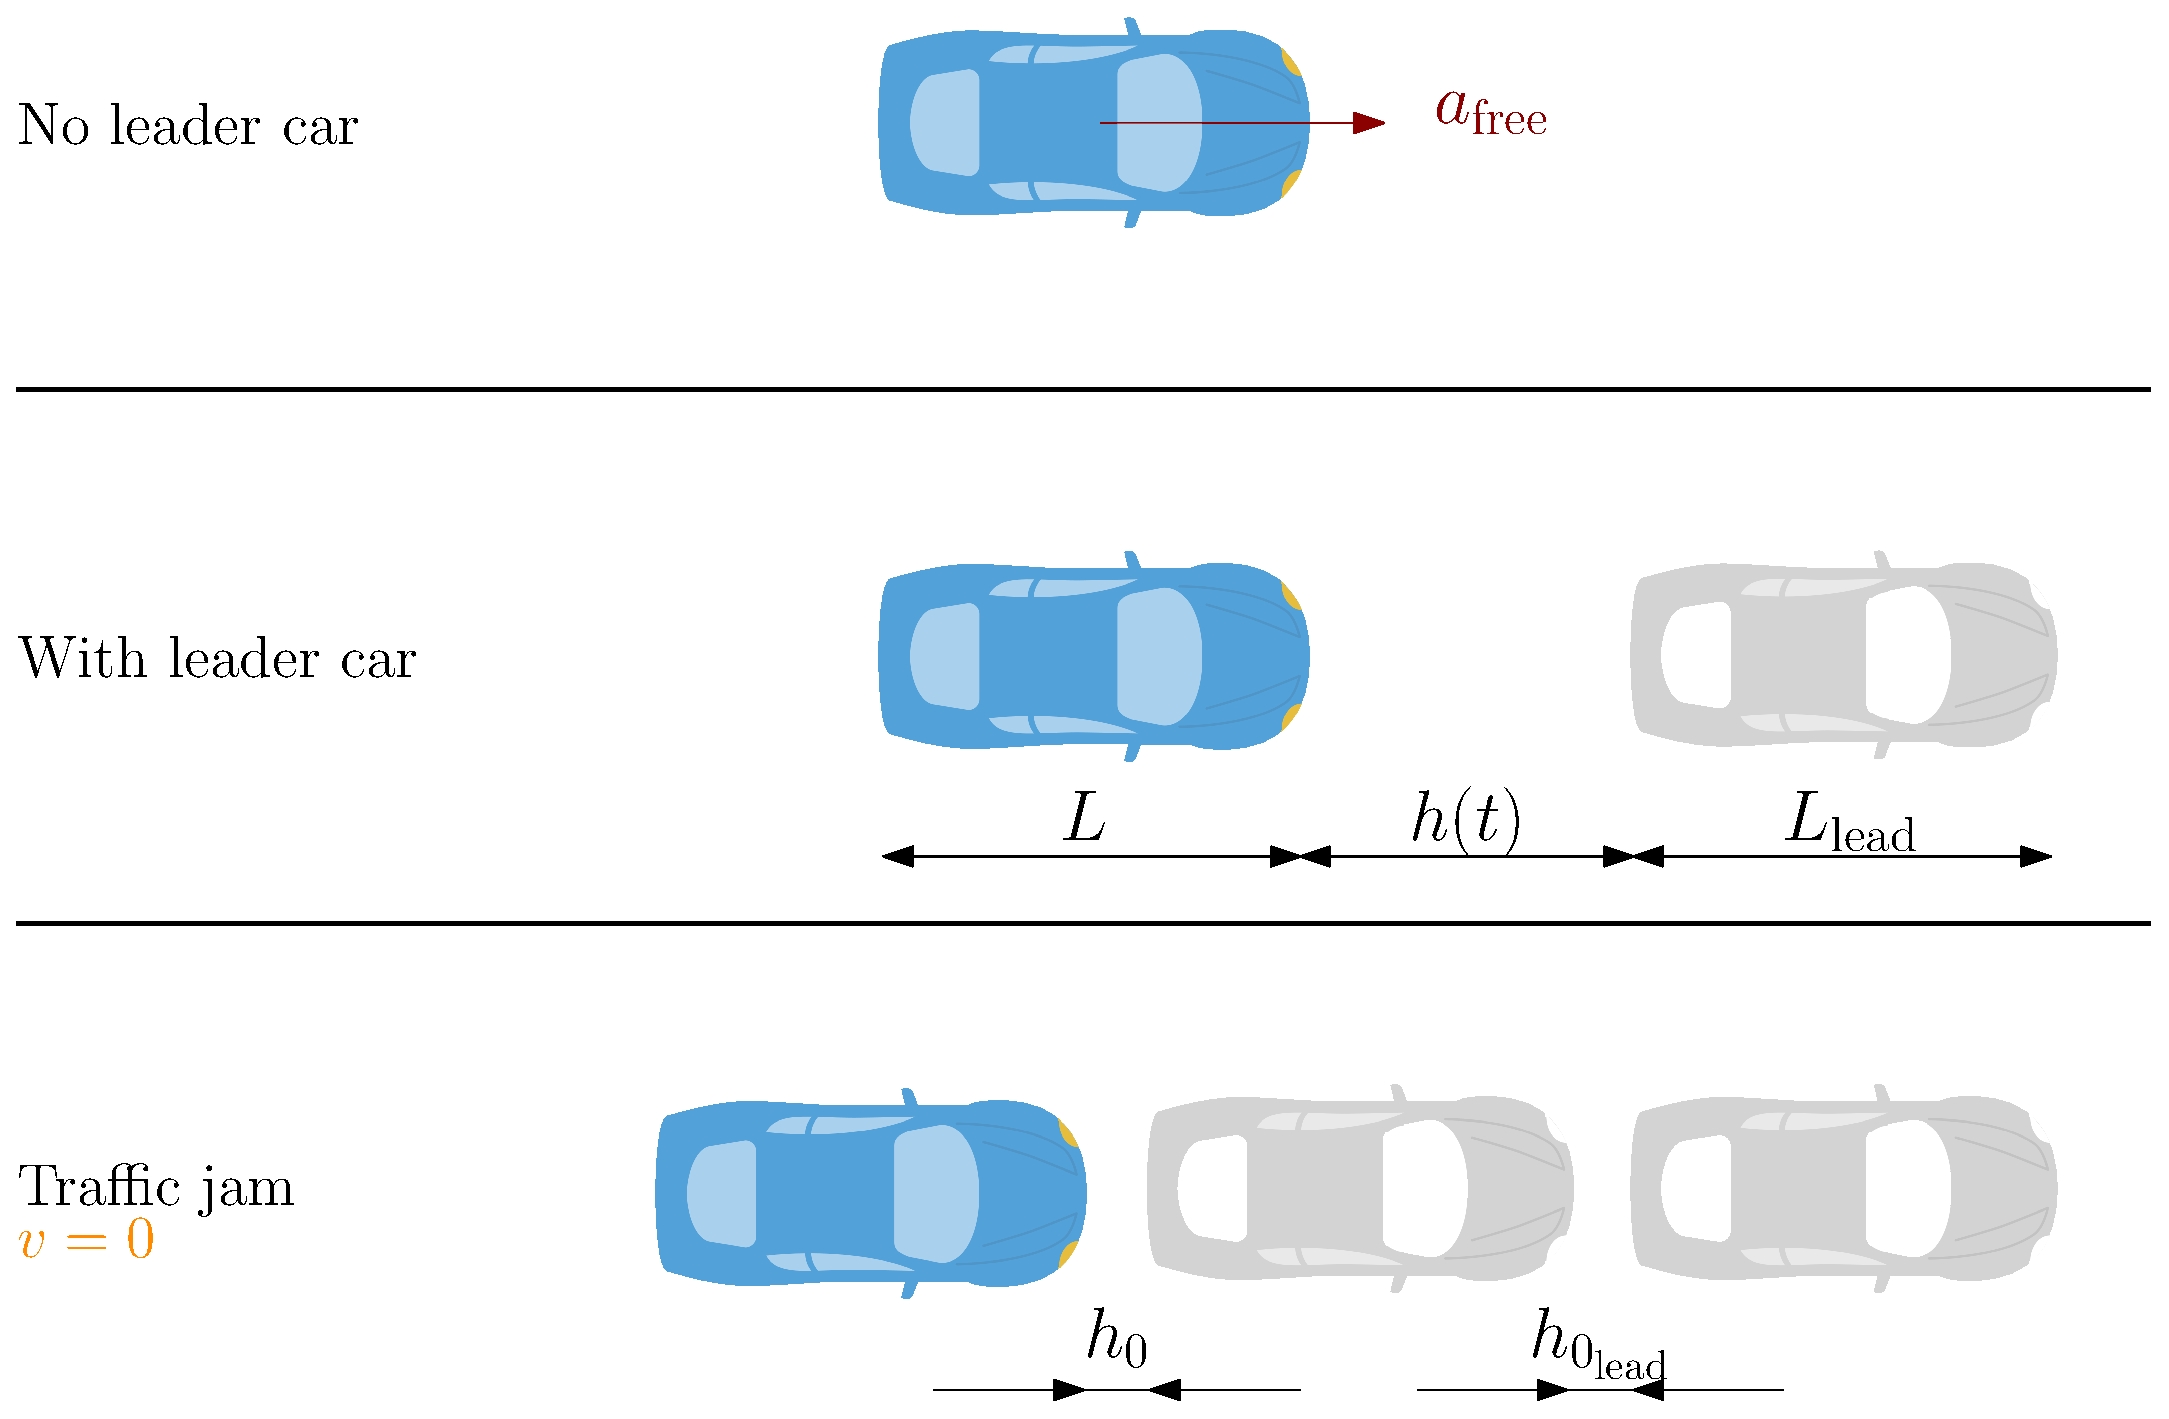
\includegraphics[width=.95\textwidth]{common/idm}
			\caption{3 cases of IDM model}
			\label{fig:idm}
		\end{figure}
		The sum of equation \ref{eq:afree} and \ref{eq:afollower} is the IDM equation which reads as follows:
		\begin{equation}
			a(t)=\afree+\afollower=\amax\left [ 1 - \left ( \frac{\vt}{\vd} \right )^{\delta} - \left ( \frac{\hd}{\h} \right )^2 \right ]\,.
			\label{eq:aidm}
		\end{equation}
		Equation \ref{eq:aidm} represents the longitudinal behavior mechanism of a human driven car. 3 cases of traffic situation were drawn on figure \ref{fig:idm} with their representative parameters.
	\section{MOBIL -- lane changing model} \label{sec:MOBIL}
		Beside the IDM there is a need for transversal motion model of the cars, namely a lane changing model. It has not been studied nearly as exhaustive as longitudinal behaviors. However it can have great impact on the overall traffic flow so it is worth investigating. The model should be able to decide based on the local traffic conditions that changing lane is beneficial and safe to a specific driver or not. If both conditions met the model will start to change lanes.

		The first condition to satisfy is that lane changing should be safe. The model should check that how will a possible lane change effect the upstream vehicles in the target lane. Mobil states if the deceleration of the new follower car does not exceed a given safe limit then changing lanes is safe. It can be expressed with an inequality as well:
		\begin{equation}
			\hat{a}_{n}\geq -b_{\rm safe}\,,
		\end{equation}
		where $\hat{a}_{n}$ is the new follower car's acceleration if car $c$ changes lanes and $b_{\rm safe}$ is a parameter of car $n$. This criterion ensures that the model remains accident free even for edge cases.
			\begin{figure}[ht]
				\centering
				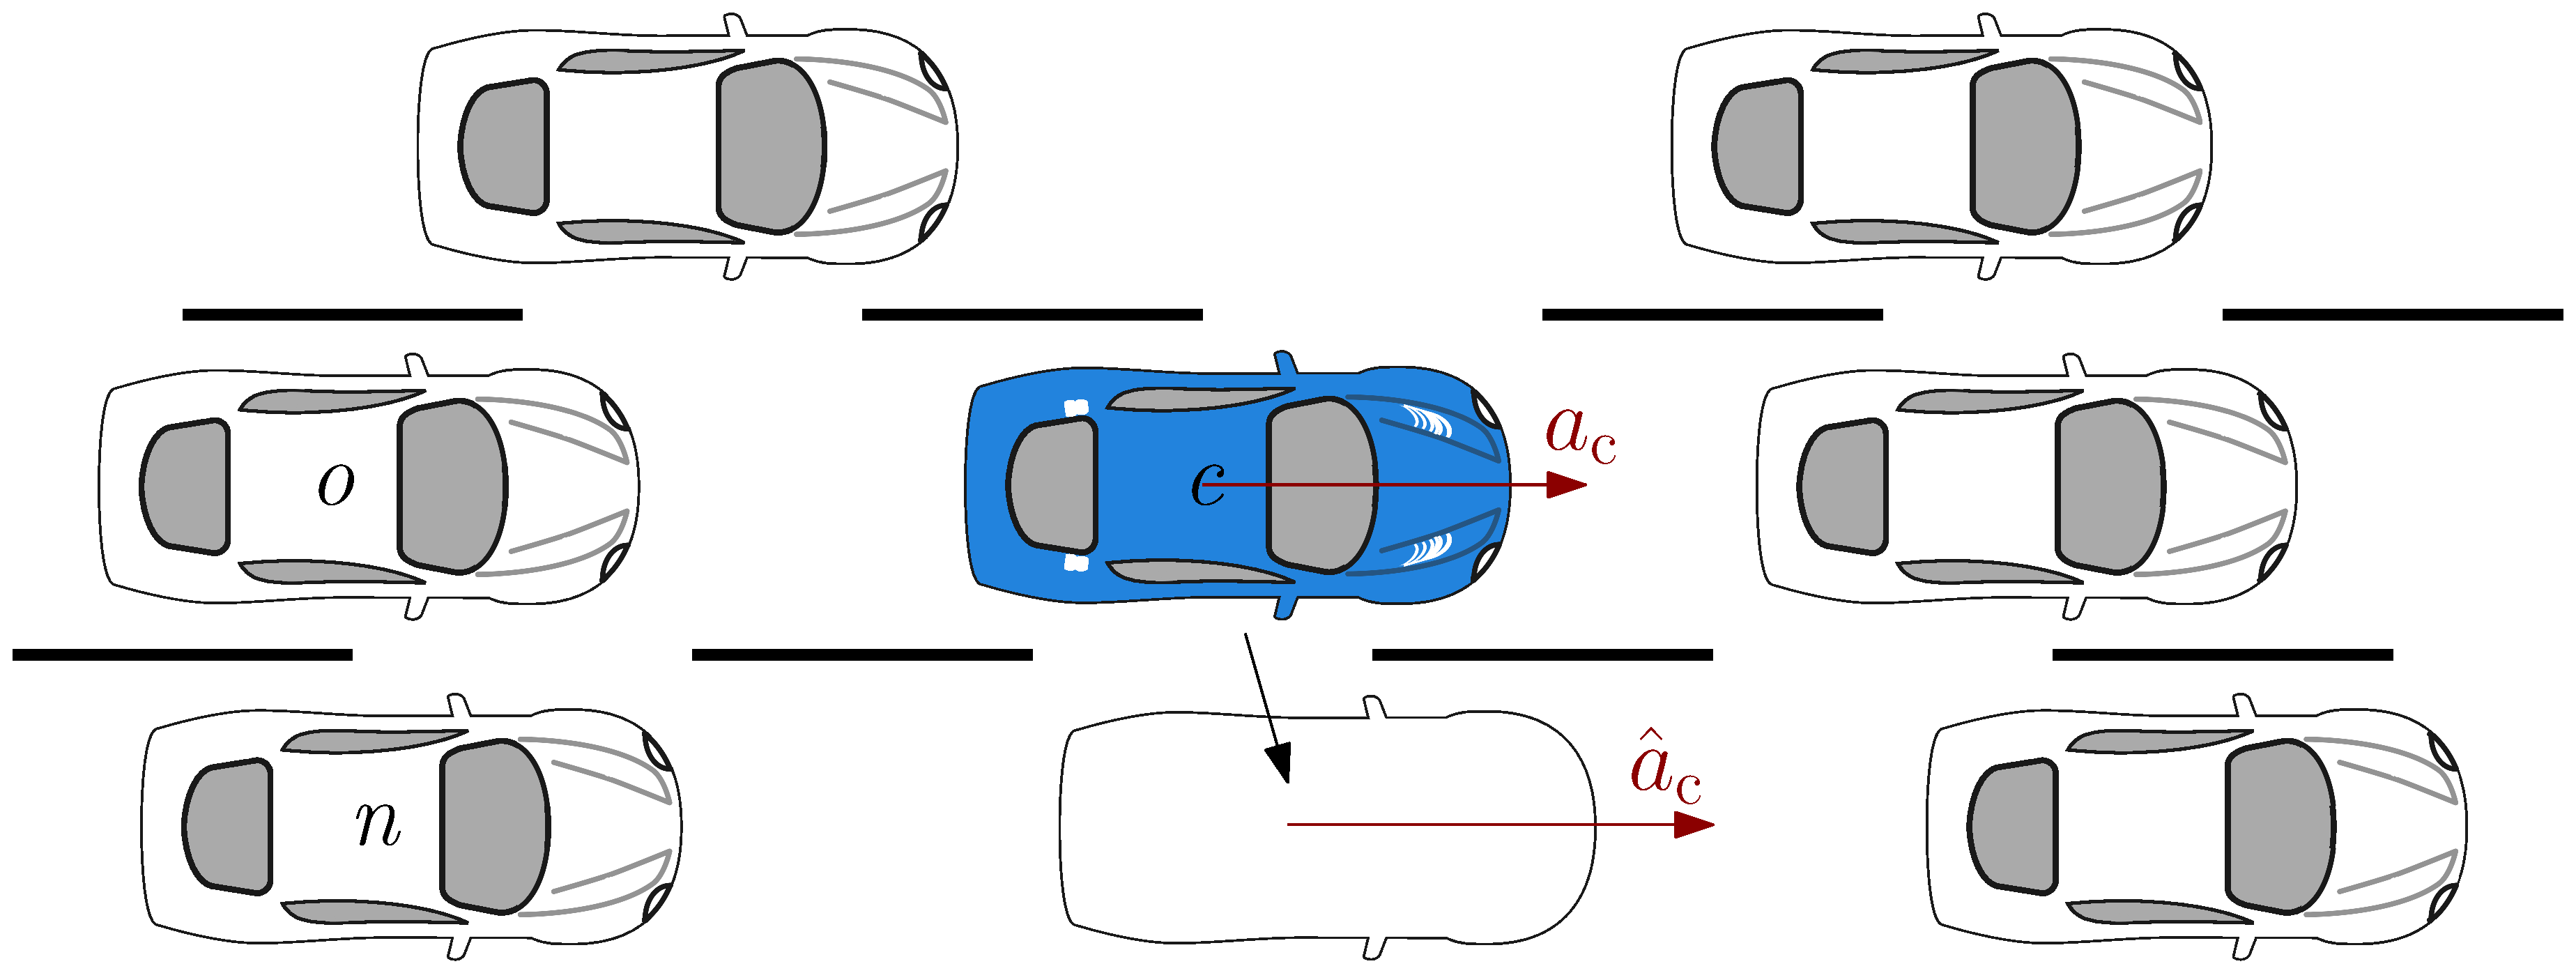
\includegraphics[width=.95\textwidth]{common/mobil}
				\caption{Based on the local traffic conditions vehicle \textit{c} is considering changing lanes  to the right. Vehicle \textit{n} and \textit{o} will be the new and old followers of car \textit{c} respectively.}
				\label{fig:mobil}
			\end{figure}
			The other condition is the incentive criterion which states that the lane change should improve the local traffic situation around the vehicle.  The base model is the following:
			\begin{equation}
				\hat{a}_{\rm c} + \hat{a}_{\rm o} + \hat{a}_{\rm n} > a_{\rm c} + a_{\rm o} + a_{\rm n}\,,
				\label{eq:mobil_first}
			\end{equation}
			where accelerations after a possible lane change are denoted with caps.
			Based on equation \ref{eq:mobil_first} a lane change should occur only if the sum of the accelerations after the lane change is greater than before. This inequality reflects the name of the model which is \textbf{m}inimizing \textbf{o}verall \textbf{b}raking \textbf{i}nduced by \textbf{l}ane change.

			However equation \ref{eq:mobil_first} is not as realistic as it should be. The first problem is that vehicles would change lanes  even for a negligible acceleration advantage which is not the case in a realistic traffic situation. This issue can be solved with a threshold value $\Delta  a_{\rm th}$. After this modification equation \ref{eq:mobil_first} would look like below:
			\begin{equation}
				\hat{a}_{\rm c} - a_{\rm c} + \hat{a}_{\rm o} - a_{\rm o} + \hat{a}_{\rm n} - a_{\rm n} > \Delta  a_{\rm th}\,,
				\label{eq:mobil_with_tr}
			\end{equation}
			It can be stated that with this modification individual drivers only change lanes if the acceleration sum is significantly greater than before the lane change. The other problem with the previously discussed model is that they can't distinguish between driving style. Driver styles can vary from complete selfish to the altruistic driver. Selfish drivers would only care about  their own acceleration ($\hat{a}_{\rm c} - a_{\rm c} > \Delta  a_{\rm th}$) while altruistic ones would change lanes even if that would result in a disadvantageous position for them but with that change the local traffic situation would improve sufficiently ($\hat{a}_{\rm o} - a_{\rm o} + \hat{a}_{\rm n} - a_{\rm n} > \Delta  a_{\rm th}$). A $p$ politeness factor should be introduced to fix that. Including $p$ in equation \ref{eq:mobil_with_tr} results in the final form of the model:
			\begin{equation}
				\hat{a}_{\rm c} - a_{\rm c} + p(\hat{a}_{\rm o} - a_{\rm o} + \hat{a}_{\rm n} - a_{\rm n}) > \Delta  a_{\rm th}\,.
				\label{eq:mobil}
			\end{equation}
			A completely selfish driver would get $p=0$ factor, while an altruistic one $p>1$. In the special case where $p=1$ equation \ref{eq:mobil} simplifies back to equation \ref{eq:mobil_with_tr}, which means a lane change is performed only if the sum of all involved vehicles' acceleration will improved at least by the threshold value.
		\section{Numerical solver}
			In Section \ref{sec:IDM} and \ref{sec:MOBIL} a vehicle behavior in traffic has been shown and modeled. The mathematical model of a driver is a second order differential equation. There is no analytical solution, so a numerical one should be carried out. To be able to use one of the common numerical solvers (like Explict Euler or 4th order Runge Kutta) the second order differential equation should be transformed into a first order differential equation system. So the second order differential equation to solve based on \ref{eq:aidm} and the facts that $v=\dot{x},\,a=\ddot{x}$, will be the following:
			\begin{equation}
				\ddot{x}=\amax\left [ 1 - \left ( \frac{\dot{x}}{\vd} \right )^\delta - \left ( \frac{h_0 + \dot{x}\cdot T + \frac{\dot{x}(\dot{x}-v_{\rm lead})}{{\rm c}}}{x_{\rm lead}-L_{\rm lead} - x} \right )^2 \right ]\,.
				\label{eq:idm_num1}
			\end{equation}
			Let's say
			\begin{equation}
				\textbf{y}=
				\begin{pmatrix}
					y_1\\
					y_2
				\end{pmatrix}
				=
				\begin{pmatrix}
					x\\
					\dot{x}
				\end{pmatrix}\,,
				\label{eq:idm_num2}
			\end{equation}
			then the derivative of $\textbf{y}$ would be
			\begin{equation}
				\dot{\textbf{y}}=
				\begin{pmatrix}
					\dot{y_1}\\
					\dot{y_2}
				\end{pmatrix}
				=
				\begin{pmatrix}
					\dot{x}\\
					\ddot{x}
				\end{pmatrix}\,,
				\label{eq:idm_num3}
			\end{equation}
			From equations \ref{eq:idm_num1}, \ref{eq:idm_num2} and \ref{eq:idm_num3} it can be concluded that the differential equation system will be the following:
			\begin{equation}
				\dot{\textbf{y}}
				=
				\begin{pmatrix}
					f_1(y_2)\\
					f_2(y_1,y_2,x_{\rm lead},v_{\rm lead})\\
				\end{pmatrix}
				=
				\begin{pmatrix}
					y_2\\
					\amax\left [ 1 - \left ( \frac{y_2}{\vd} \right )^{\delta} - \left ( \frac{h_0 + y_2\cdot T + \frac{y_2(y_2-v_{\rm lead})}{{\rm c}}}{x_{\rm lead} - L_{\rm lead} - y_1} \right )^2 \right ]
				\end{pmatrix}
				\label{eq:numerical_idm}
			\end{equation}
	\chapter{Evolution of the simulator}
	\section{Basic 2 car setup with IDM}\label{sec:base2car}
		Equation \ref{eq:numerical_idm} can be solved with an Explicit Euler. To test the model a basic setup was implemented in MATLAB. The visual representation of the setup can be seen on figure \ref{fig:basic2car}.
		\begin{figure}[ht]
			\centering
			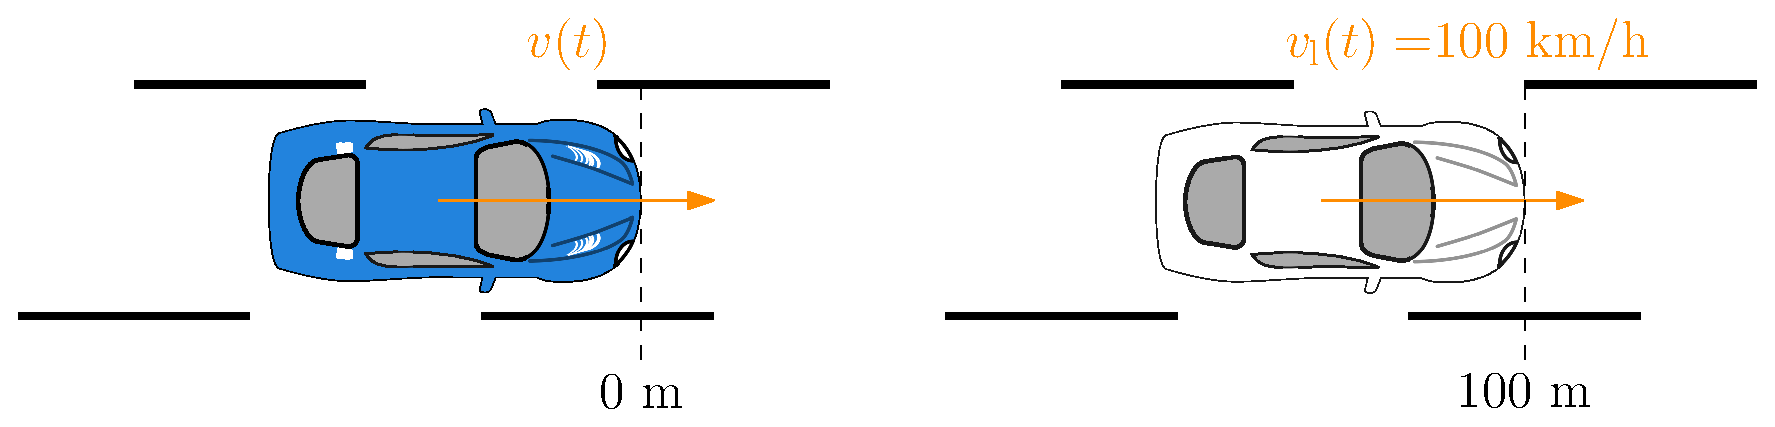
\includegraphics[width=.95\textwidth]{common/basic_2_car}
			\caption{Basic setup with 2 cars}
			\label{fig:basic2car}
		\end{figure}
		The leading car has a constant 100 km/h velocity. The following car - which is modeled with IDM - has an initial velocity of 100 km/h as well. The second car is 100 meters behind the other car. The parameters of following car can be seen in Table \ref{tab:idm_params}. The parameters have been chosen based on literature from [TODO:reference here].
		\begin{table}[ht]
			\begin{center}
				\begin{tabular}{ |c|c|c| }
					\hline
					$a_{\rm max}$ & $1.5$ & $\rm m/s^2$ \\
					$b_{\rm max}$ & $1.67$ & $\rm m/s^2$ \\
					$v_{\rm d}$ & $130$ & km/h \\
					$T$ & $1.8$ & s \\
					$h_0$ & $2$ & m \\
					$\rm \delta$ & $4$ & - \\
					$L$ & $4.5$ & m \\
					\hline
				\end{tabular}
			\end{center}
			\caption{Intelligent Driver Model parameters}
			\label{tab:idm_params}
		\end{table}
		The simulation was run until 100 seconds. Figure \ref{fig:basic2car_case_1} shows the result. The initial gap between the cars is greater than the second car's desired headway, consequently the vehicle will accelerate. The gap between the vehicles starts to decrease. At a certain time (around $t =$ 10) the second car starts to decelerate slowly based on the velocity difference and the decreasing headway. It will reach the desired safe gap at some point and will have exactly the same speed as the car before. It will maintain its desired headway.
		\begin{figure}[ht]
			\centering
			\begin{minipage}{.5\textwidth}
				\centering
				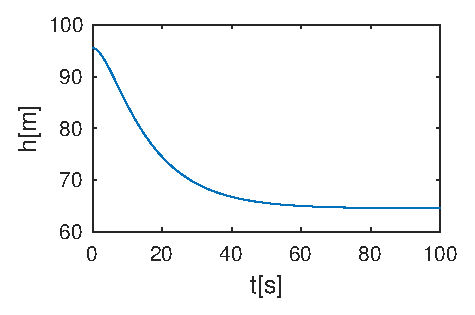
\includegraphics{ee/basic_2_car_headaway_case_1_2}
			\end{minipage}\hfill
			\begin{minipage}{.5\textwidth}
				\centering
				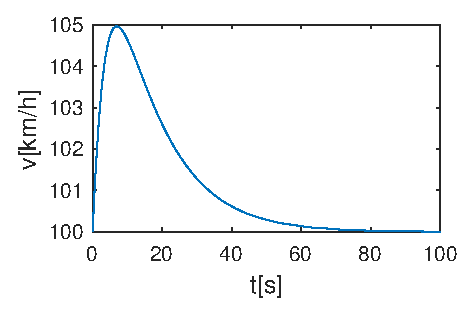
\includegraphics{ee/basic_2_car_velocity_case_1_2}
			\end{minipage}
			\caption{Following car's headway and velocity in Setup 1}
			\label{fig:basic2car_case_1}
		\end{figure}

		Another simulation was run with the same configuration except that the first car's front is set to be at 40 meters instead of 100. Figure \ref{fig:basic2car_case_2} shows the result. In this case the gap between cars is less than the second vehicle's desired safety headway. So it will decelerate first than accelerate to reach the desired gap. Fundamentally the same happened but in the opposite direction.
		\begin{figure}[ht]
			\centering
			\begin{minipage}{.5\textwidth}
				\centering
				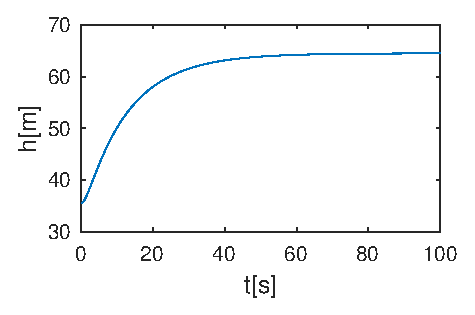
\includegraphics{ee/basic_2_car_headaway_case_2_2}
			\end{minipage}\hfill
			\begin{minipage}{.5\textwidth}
				\centering
				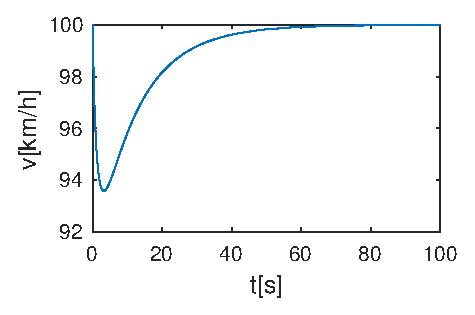
\includegraphics{ee/basic_2_car_velocity_case_2_2}
			\end{minipage}
			\caption{Following car's headway and velocity in Setup 2}
			\label{fig:basic2car_case_2}
		\end{figure}
		Both examples showed that the stationary state does not depend on the initial gap. After a little bit of time the second car has reached the desired safety gap (which is around 64.5 meters) and the 100 km/h speed in both cases.
	\section{Model behavior verification}
		In Section \ref{sec:base2car} two examples were shown where the model produced the same stationary state for different initial conditions. Stationary state means that the vehicle's acceleration is zero. So equation \ref{eq:aidm} modifies as followings in a stationary state:
		\begin{equation}
		1 - \left ( \frac{v_{\rm stac}}{v_{\rm d}} \right )^{\rm \delta} - \left ( \frac{h_0+v_{\rm stac}\cdot T+\frac{v_{\rm stac}(v_{\rm l,stac}-v_{\rm stac})}{2\sqrt{\amax \bmax}}}{x_{\rm l,0}+v_{\rm l, stac}\cdot t-x_{0} - L_{\rm l} + v_{\rm stac}\cdot t} \right )^2=0\,,
		\label{eq:aidm_stac1}
		\end{equation}
		There is an other consequence of this situation as well. As it can be seen in the examples, cars' velocities were equal, which means:
		\begin{equation}
			v_{\rm stac}=v_{\rm l,stac}\,,
		\end{equation}
		so Equation \ref{eq:aidm_stac1} will further simplifies to:
		\begin{equation}
			1 - \left ( \frac{v_{\rm stac}}{v_{\rm d}} \right )^{\rm \delta} - \left ( \frac{h_0+v_{\rm stac}\cdot T}{x_{\rm l,0}-x_{0} - L_{\rm l}} \right )^2=0\,.
		\end{equation}
		It can be stated that the stationary gap between the vehicles equals to the denominator of the second fraction expression:
		\begin{equation}
		1 - \left ( \frac{v_{\rm stac}}{v_{\rm d}} \right )^{\rm \delta} - \left ( \frac{h_0+v_{\rm stac}\cdot T}{h_{\rm stac}} \right )^2=0\,.
		\label{eq:aidm_stac2}
		\end{equation}
		Expression \ref{eq:aidm_stac2} shows that $v_{\rm stac}$ only depends on $h_{\rm stac}$. Everything else in the equation is a parameter of the model. Consequently every stationary gap has a corresponding speed value. Plot of Equation \ref{eq:aidm_stac2} can be seen on Figure \ref{fig:aidm_stac}.% [TODO: check this figure error, it hides half of the line before]
		\begin{figure}[ht]
			\centering
			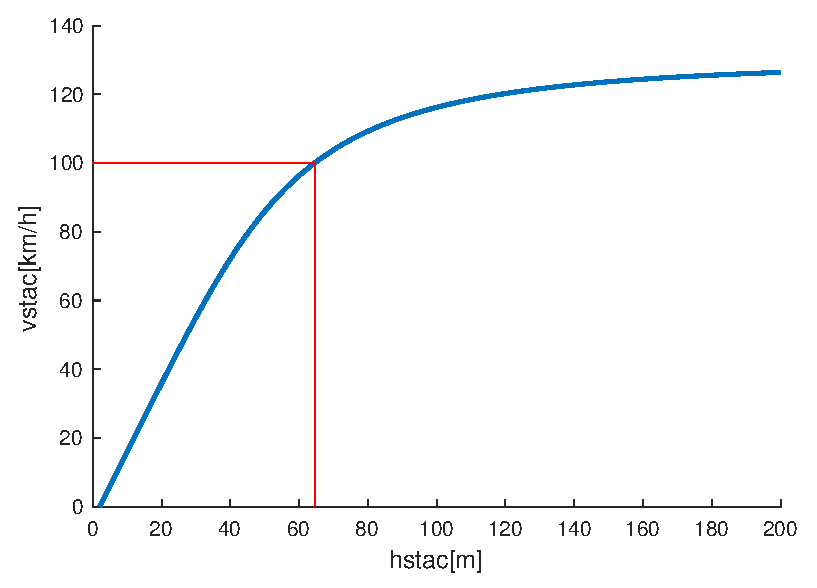
\includegraphics{check/check_stationary_states}
			\caption{Stationary velocity based on stationary headway}
			\label{fig:aidm_stac}
		\end{figure}
	\chapter{Final model}
	\section{Blending the IDM and MOBIL}
		Until this point all simulations were run in a one lane imaginary road. However to be able to represent real traffic situations multi lane roads has to be considered as mentioned in the introduction. In a multi lane road IDM can describe the longitudinal and MOBIL the transversal motions. For a starting point let us revisit the model used previously:
		\begin{equation}
			\dot{y}=
			\begin{pmatrix}
			v_0\\
			0\\
			f_1(v_{2})\\
			f_2(x_{2}, v_{2},x_{1}, v_{1})\\
			f_1(v_{3})\\
			f_2(x_{3}, v_{3},x_{2}, v_{2})\\
			\vdots\\
			f_1(v_{\rm n-1})\\
			f_2(x_{n-1}, v_{n-1},x_{n-2}, v_{n-2})\\
			f_1(v_{\rm n})\\
			f_2(x_{n}, v_{n},x_{n-1}, v_{n-1})
			\end{pmatrix}\,.
			\label{eq:n_ode_math_revisit}
		\end{equation}
		As Equation \ref{eq:n_ode_math_revisit} shows there is a criterion on the car indexing.  Namely ($n-1$)-th vehicle is always the leader of $n$-th car. Every car is stored in an array called definition array with their identifiers,  current and target lanes, initial positions and velocities, and parameters. An example of this definition array can be seen in Table \ref{tab:definition_array}.
		\begin{table}
			\begin{center}
				\begin{tabular}{ |c|c|c|c|c|c| }
					\hline
					Id & Current lane & Target lane & Initial position & Initial velocity& IDM params\\
					$[-]$ & $[-]$ & $[-]$ & $[m]$ & $[m/s]$ & $[-]$\\
					\hline
					1 & 1 & 0 & 100 & 0 & ...\\
					2 & 2 & 0 & 50 & 0 & ...\\
					\vdots & \vdots & \vdots & \vdots & \vdots & \vdots\\
					n - 1 & 1 & 0 & 200 & 0 & ...\\
					n & 1 & 0 & 0 &  & ...\\
					\hline
				\end{tabular}
			\end{center}
			\caption{Definition array example}
			\label{tab:definition_array}
		\end{table}
		Since there were no lane changes until this point,the indexing condition held. However this criterion cannot be satisfied where changing lanes are allowed. Instead of this condition a new function is introduced. The suggested method is capable of calculating which car is the leader of an other vehicle. So from now on the simulator relies on this function instead of the order of car models in the definition array.
		\subsection*{Determining the leader vehicle}
		The previously mentioned function does the following steps
		\begin{itemize}
			\item assembles and sorts a car model array with the required data by current vehicle position,
			\item searches for cars in the same lane,
			\item finds the row of the car by id,
			\item returns the row above (index - 1) if exists or nothing if there is no row above.
		\end{itemize}
		Let us call this function $g$. This $g$ function has one parameter, the id of the car whose leader vehicle is searched for. If there is leader than it returns exactly the same values as the IDM expects as parameters, namely the leading car's position and velocity.
		So Equation \ref{eq:n_ode_math_revisit} modifies as follows:
		\begin{equation}
			\dot{y}=
			\begin{pmatrix}
			v_0\\
			0\\
			f_1(v_2)\\
			f_2(x_{2}, v_{2},g(\id_2))\\
			f_1(v_2))\\
			f_2(x_{3}, v_{3},g(\id_3))\\
			\vdots\\
			f_1(v_{n-1}))\\
			f_2(x_{n-1}, v_{n-1},g(\id_{n-1}))\\
			f_1(v_n))\\
			f_2(x_{n}, v_{n},g(\id_{n}))
			\end{pmatrix}\,.
			\label{eq:n_ode_math_with_find_leading}
		\end{equation}
		As mentioned previously $g$ function can only return the expected parameters by $f$ if there is a leader car. This makes sense since someone has to be the very first in every single time step. Consequently that cars longitudinal model has to be changed to handle that there is no car in front of it. It is handled by leaving the follower behavior out of the equation \ref{eq:aidm}. So it will not need the leader vehicle's parameters. This means that the leader cars in their lanes will always be in free acceleration state. That is coinciding with reality.
		\subsection*{Implementation of lane changing}
		The original n-car solver only calculated and stored the \textbf{y} vector which contained the position and velocity values at each time step. Since lane changes came into picture that wont be enough. Consequently, two more vectors needs to be stored. One for the current lane (named $\vcl$) and one for the target lane (named $\vtl$) which can keep track of the lane changes. $\vcl$ will store the lane numbers of the vehicle's current lane. $\vtl$ will contain the target lane identifier when a car is changing lane, otherwise it will have zero value. Figures \ref{fig:stage1ofchanginglanes}, \ref{fig:stage2ofchanginglanes}, \ref{fig:stage3ofchanginglanes} show the stages of a lane change example.
		\begin{figure}
			\begin{center}
				\begin{minipage}{.65\textwidth}
					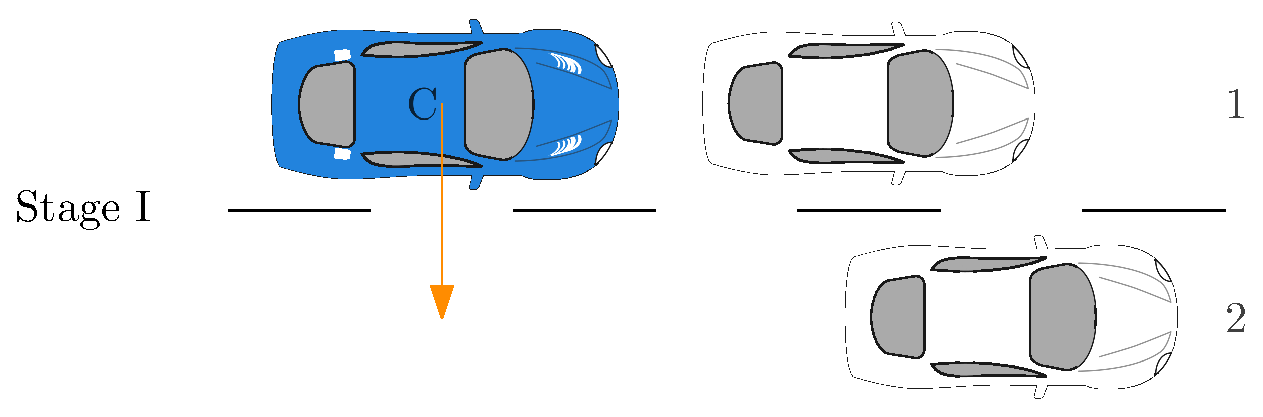
\includegraphics[width=\textwidth]{common/stages_of_lane_changes_1}
				\end{minipage}\quad
				\begin{minipage}{.3\textwidth}
					\begin{tabular}{ |c|c|c|c| }
						\hline
						Id &  $\vcl$ & $\vtl$ & ... \\
						$[-]$ & $[-]$ & $[-]$ & ...\\
						\hline
						$\vdots$ & $\vdots$ & $\vdots$ & \vdots\\
						$C$ & $1$ & $0$ & ...\\
						$\vdots$ & $\vdots$ & $\vdots$ & \vdots\\
						\hline
					\end{tabular}
				\end{minipage}
			\end{center}
			\caption{Stage I of changing lanes. Vehicle C is considering a lane change.}
			\label{fig:stage1ofchanginglanes}
		\end{figure}
		\begin{figure}
			\begin{center}
				\begin{minipage}{.65\textwidth}
					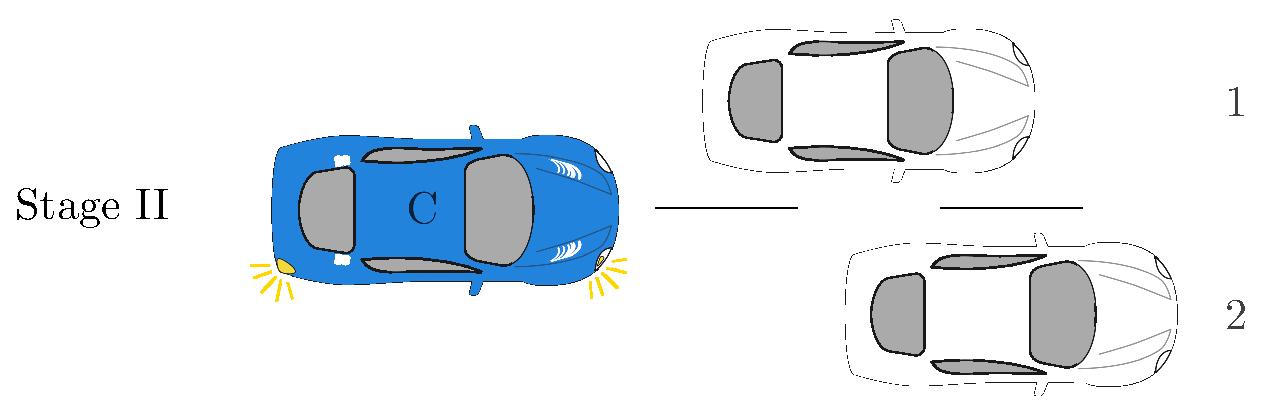
\includegraphics[width=\textwidth]{common/stages_of_lane_changes_2}
				\end{minipage}\quad
				\begin{minipage}{.3\textwidth}
					\begin{tabular}{ |c|c|c|c| }
						\hline
						Id &  $\vcl$ & $\vtl$ & ... \\
						$[-]$ & $[-]$ & $[-]$ & ...\\
						\hline
						$\vdots$ & $\vdots$ & $\vdots$ & \vdots\\
						$C$ & $1$ & $2$ & ...\\
						$\vdots$ & $\vdots$ & $\vdots$ & \vdots\\
						\hline
					\end{tabular}
				\end{minipage}
			\end{center}
			\caption{Stage II of changing lanes. Vehicle C changing lanes from lane 1 to lane 2. The row of vehicle C contains 1 in the current lane vector and 2 in the target lane vector.}
			\label{fig:stage2ofchanginglanes}
		\end{figure}
		\begin{figure}[ht]
			\begin{center}
				\begin{minipage}{.65\textwidth}
					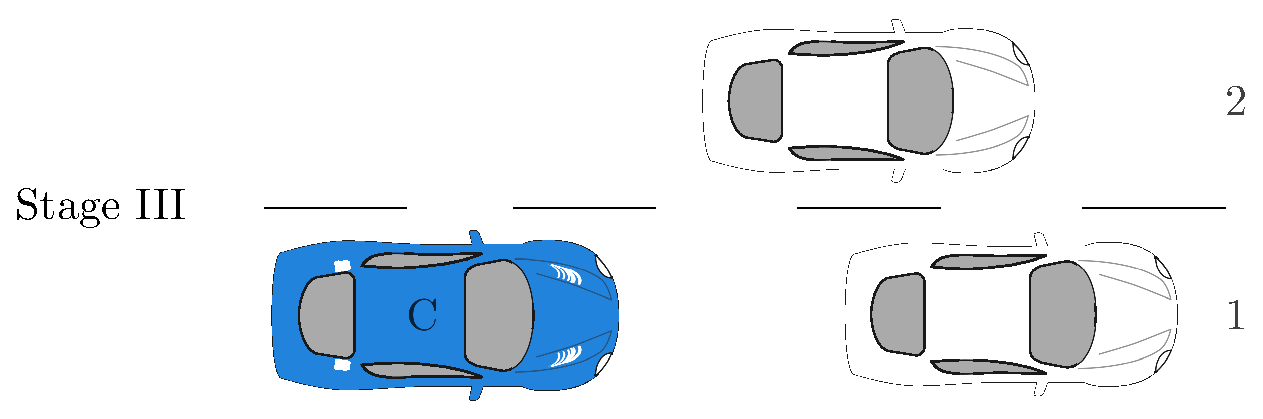
\includegraphics[width=\textwidth]{common/stages_of_lane_changes_3}
				\end{minipage}\quad
				\begin{minipage}{.3\textwidth}
					\begin{tabular}{ |c|c|c|c| }
						\hline
						Id &  $\vcl$ & $\vtl$ & ... \\
						$[-]$ & $[-]$ & $[-]$ & ...\\
						\hline
						$\vdots$ & $\vdots$ & $\vdots$ & \vdots\\
						$C$ & $2$ & $0$ & ...\\
						$\vdots$ & $\vdots$ & $\vdots$ & \vdots\\
						\hline
					\end{tabular}
				\end{minipage}
			\end{center}
			\caption{Stage III of changing lanes. Vehicle C has performed its lane change so the current lane vector will hold a value of 2 at the row of vehicle C, corresponding row of target lane vector will reset to zero.}
			\label{fig:stage3ofchanginglanes}
		\end{figure}
		\subsection*{Decision making and duration of a lane change}
		The updated model with vectors $\vcl$ and $\vtl$ is able to keep track of a multi lane traffic with lane changes. However the algorithm to fill those vectors correctly is not discussed yet. A lane change has multiple aspects like when does the driver wants to change, is it possible change lanes safely, how much time does it take. Fortunately the first two question can be answered by simply implementing the algorithm of MOBIL. However the duration of a lane change must be implemented elsewhere.

		From the implementation point of view in every time step MOBIL calculates that should a driver change lanes or not. If a driver should change lanes based on the local traffic situation than the lane change starts by filling the corresponding row in the vector $\vtl$. The actual duration of the lane change should be defined as a driver parameter in seconds. A typical value is 2 to 3 sec. After a lane change has started the simulator is checking the elapsed time in every time step for the corresponding vehicle. When the elapsed time has exceeded the lane change duration then car's current lane value will be the target lane value and target lane resets to zero. It is worth mentioning that a lane changing car occupies both its current and target lane. So it will be the leader car in both current and target lane's immediate following cars.
	\section{Simulation of a traffic light situation}
		The model described in the previous section has been implemented in \textsc{Matlab}. The task is to test the solver through an interesting case like a red traffic light with 10 vehicles.
		\subsection*{Initial conditions}
		The initial conditions can be found in Table \ref{tab:case_1_definition_array}. The traffic situation can be seen on Figure \ref{fig:red_light_situation}. The front of the first car of each lane has been placed at zero position. Then every vehicle has been behind its leader by its traffic jam distance. The initial velocity of all cars is zero.  The IDM parameters of the simulated cars have been varied between realistic values. Also for the first time a bus has been introduced to traffic. From the model point of view a bus is only different from a regular car by its length and some of its IDM parameters like the maximum acceleration or duration of a lane change.
		\begin{table}
			\begin{center}
				\begin{tabular}{ |c|c|c|c|c|c| }
					\hline
					Id & Current lane & Target lane & Initial position & Initial velocity& IDM params\\
					$[-]$ & $[-]$ & $[-]$ & $[m]$ & $[m/s]$ & $[-]$\\
					\hline
					1 & 1 & 0 & 0 & 0 & ..., L = 4.2, ... \\
					2 & 2 & 0 & 0 & 0 & ..., L = 4.4, ... \\
					3 & 1 & 0 & -5.4 & 0 & ..., L = 20, ... \\
					4 & 2 & 0 & -5.5 & 0 & ..., L = 4.1, ... \\
					5 & 1 & 0 & -26.4 & 0 & ..., L = 4.3, ... \\
					6 & 2 & 0 & -10.9 & 0 & ..., L = 4.5, ... \\
					7 & 1 & 0 & -31.9 & 0 & ..., L = 4.6, ... \\
					8 & 2 & 0 & -16.5 & 0 & ..., L = 4.2, ... \\
					9 & 1 & 0 & -37.7 & 0 & ..., L = 4.3, ... \\
					10 & 2 & 0 & -21.7 & 0 & ..., L = 4.4, ... \\
					\hline
				\end{tabular}
			\end{center}
			\caption{Initial conditions of Case 1}
			\label{tab:case_1_definition_array}
		\end{table}
		\begin{figure}
			\centering
			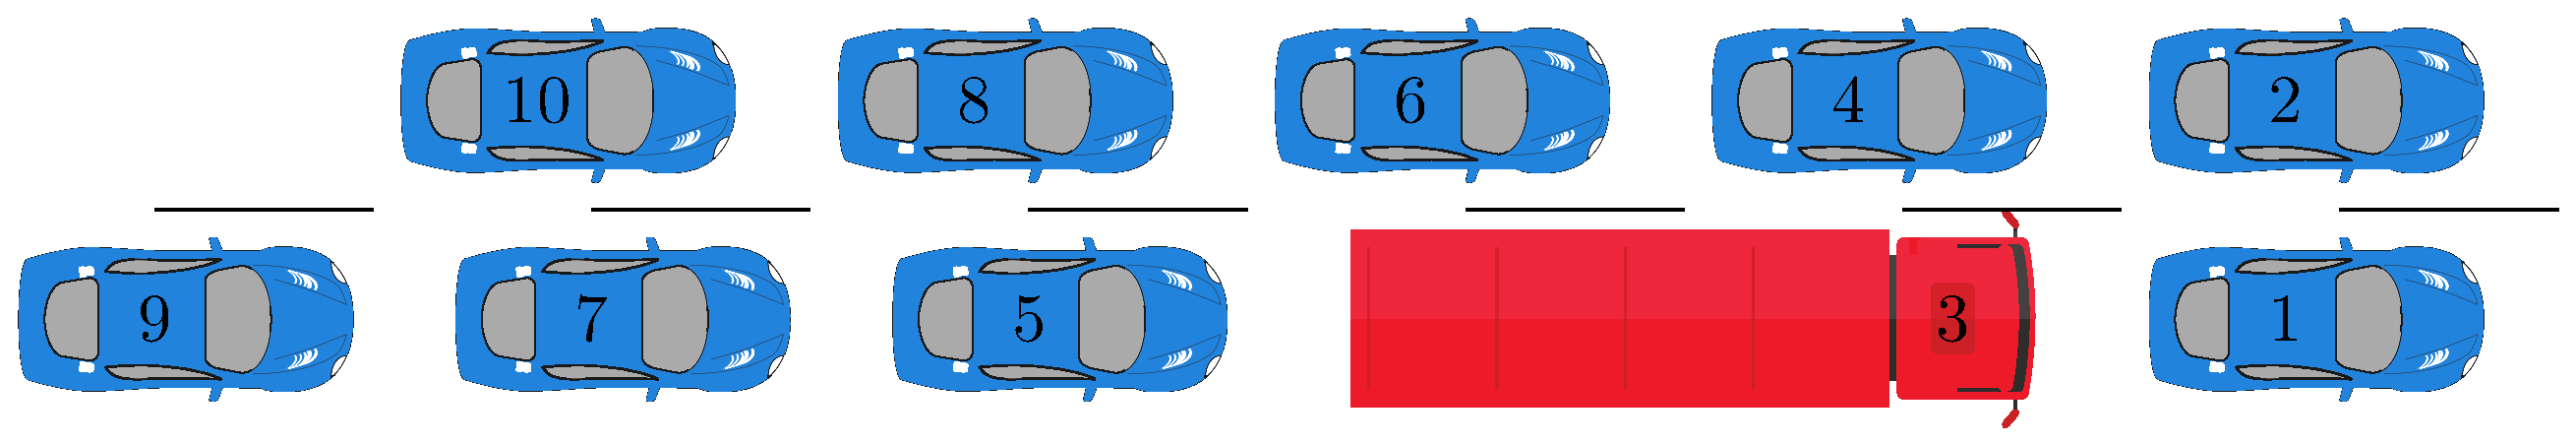
\includegraphics[width=\textwidth]{common/traffic_light_case_1}
			\caption{Red light situation with 10 vehicles}
			\label{fig:red_light_situation}
		\end{figure}
		\begin{figure}
			\centering
			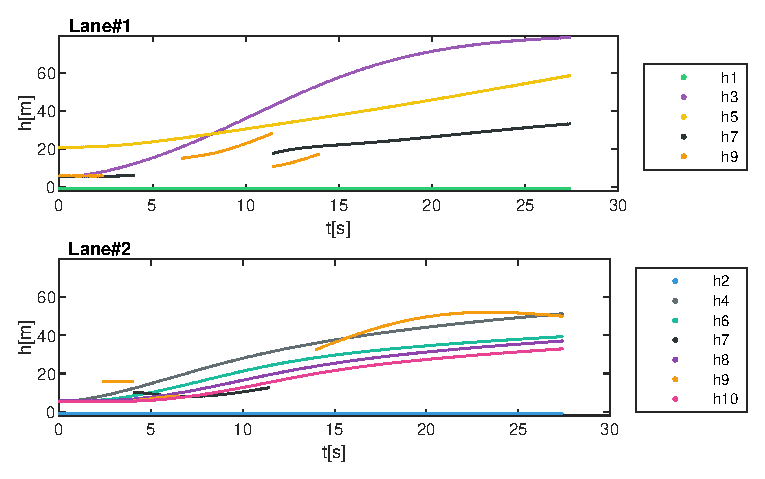
\includegraphics[width=0.8\textwidth]{eemobil/simh_case1}
			\caption{Red light traffic. Headway of the vehicles respect to their position in lanes}
			\label{fig:red_light_situationh}
		\end{figure}
		\begin{figure}
			\centering
			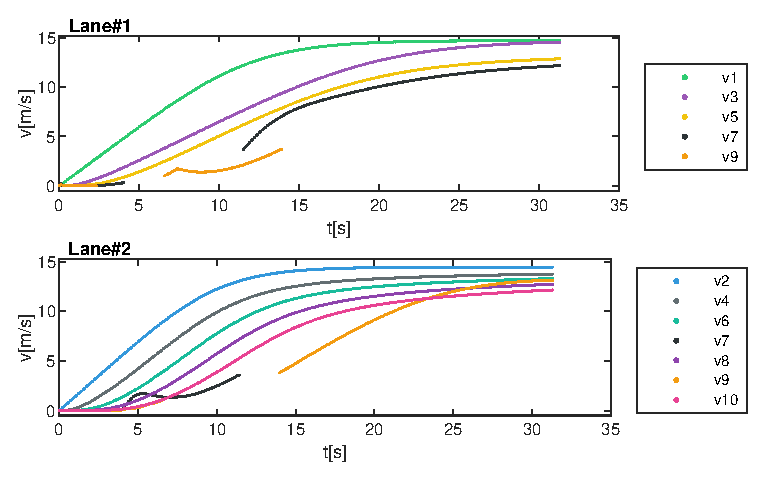
\includegraphics[width=0.8\textwidth]{eemobil/simv_case1}
			\caption{Red light traffic. Velocity of the vehicles respect to their position in lanes}
			\label{fig:red_light_situationv}
		\end{figure}
		\begin{figure}
			\centering
			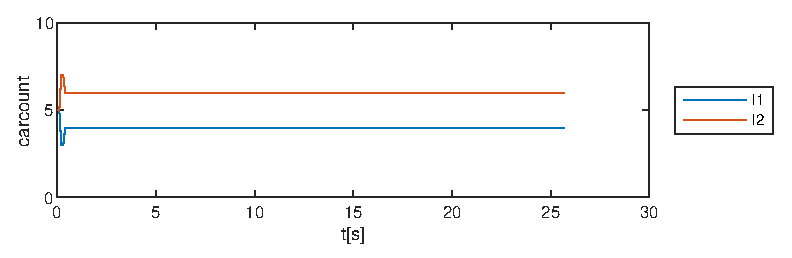
\includegraphics[width=0.8\textwidth]{eemobil/simcc_case1}
			\caption{Red light traffic. Number of cars in lanes }
			\label{fig:red_light_situationcc}
		\end{figure}
		\subsection*{Summary of the result}
		The traffic situation was successfully simulated. However post processing of the result turned out to be kind of a challenging task. The usage of the previous figures is not illustrating enough the traffic. To make it easy to understand the motions of the vehicles, the headway and velocity figures have been divided into two parts. One figure shows the headway of the cars in one lane the other figure shows the other lane. When a vehicle changes lanes its curve breaks and disappears from one figure and continues on the other. The headway and velocity diagrams can be seen on Figure \ref{fig:red_light_situationh} and \ref{fig:red_light_situationv}. Notice that the first cars of each lanes have zero headway since there is no vehicle in front of them.  Another figure was made to emphasize the lane changes during the simulation. Figure \ref{fig:red_light_situationcc} shows the number of vehicles in each lane. Notice that one function is reflections\textbf{?!} of the other.
		\section{Effect of the time step size on solutions}
		A numerical solution should be independent from the time step. Thus a time step independence analysis has been carried out. What practically it means is that one particular simulation should be run multiple times with decreasing step size. If the solution is converged than it can be said that the model is step size independent. The default value of the step size was 0.1 second. The simulations were run with the values defined in Table \ref{tab:timestepsizes}.
		Using the same parameters and initial conditions as before, the analysis has been performed. The result can be seen on Figure \ref{fig:tsip}, \ref{fig:tsiv}, \ref{fig:tsipr}, \ref{fig:tsivr} and \ref{fig:tsit}.
		\begin{figure}
			\centering
			\begin{minipage}{.5\textwidth}
				\centering
				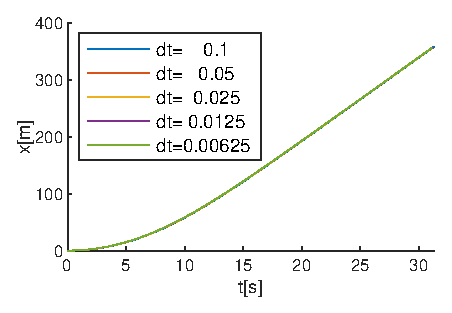
\includegraphics{eemobil/timestepi_p}
				\caption{Position of car 5}
				\label{fig:tsip}
			\end{minipage}\hfill
			\begin{minipage}{.5\textwidth}
				\centering
				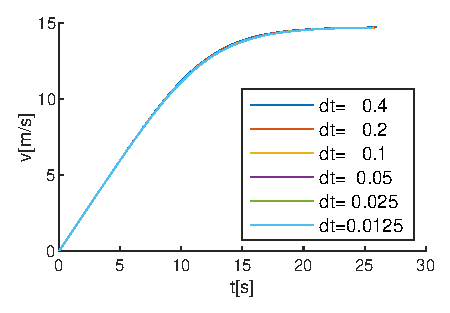
\includegraphics{eemobil/timestepi_v}
				\caption{Velocity of car 5}
				\label{fig:tsiv}
			\end{minipage}
		\end{figure}
		\begin{figure}
			\centering
			\begin{minipage}{.5\textwidth}
				\centering
				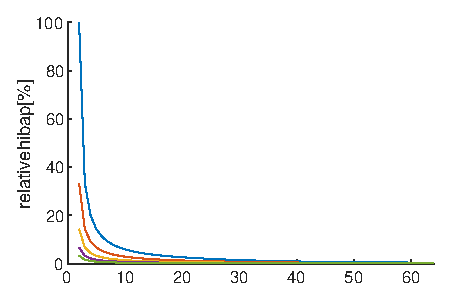
\includegraphics{eemobil/timestepi_relative_p}
				\caption{Relative error of position}
				\label{fig:tsipr}
			\end{minipage}\hfill
			\begin{minipage}{.5\textwidth}
				\centering
				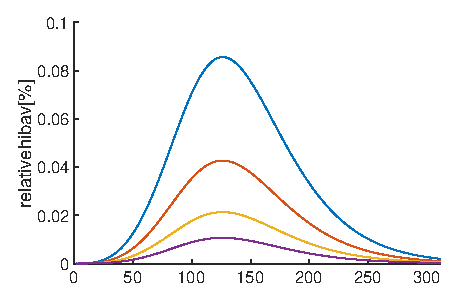
\includegraphics{eemobil/timestepi_relative_v}
				\caption{Relative error of velocity}
				\label{fig:tsivr}
			\end{minipage}
		\end{figure}
		\begin{figure}
			\centering
			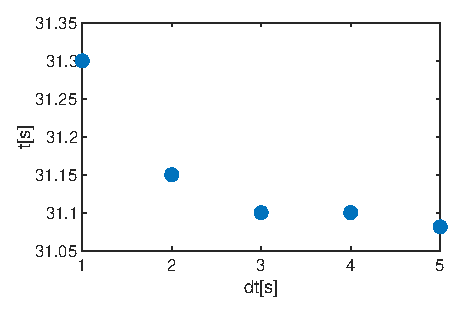
\includegraphics{eemobil/timestepi_t}
			\caption{Time step independence. Elapsed time for 100 meters}
			\label{fig:tsit}
		\end{figure}
		\begin{table}
			\begin{center}
				\begin{tabular}{ |c||c|c|c|c|c| }
					\hline
					&1. & 2. & 3. & 4. & 5.\\
					\hline
					dt[s]& $0.1$ & $0.05$ & $0.025$ & $0.0125$ & $0.00625$ \\
					\hline
				\end{tabular}
			\end{center}
			\caption{Step sizes}
			\label{tab:timestepsizes}
		\end{table}
		\section{Multi lane traffic simulator improvements}
		The simulator works as expected. It is capable of simulating a multi lane traffic with lane changes. But there are some driver behaviors that can be modeled slightly better, thus making the simulator  more realistic.
		\subsection*{Improvement I ?!!!!!!}
		Currently the acceleration value of a vehicle during a lane change is calculated by its leader only. However in a real situation a driver changes lane because he would like to accelerate. So instead of calculating the acceleration based on the current leader only, both the current and the future leader accelerations should take into account. A reasonable approximation could be that the car's current acceleration is a weighted average by the elapsed time from the duration of the lane change between the acceleration value of the current and  future leader. A mathematical expression of this improvement would look like:
		\begin{equation}
			a=a_{\rm c} \cdot \left(1-\frac{t_{\rm e}}{t_{\rm d}}\right) + a_{\rm f}\cdot \frac{t_{\rm e}}{t_{\rm d}}\,,
			\label{eq:weighted_average}
		\end{equation}
		where $a_{\rm c}$ is the acceleration considering only the current leader vehicle, $a_{\rm f}$  is the acceleration considering only the future leader vehicle. $t_e$ and $t_d$ is the elapsed and total time of the lane change. Based on Equation \ref{eq:weighted_average} the improvement has been implemented in the simulator. This feature has been added with a toggle if one wishes to turn off in the future.
		\subsection*{Improvement II}
		The other area which can be developed is related to the attention of the drivers to the road. The model currently assumes that everyone is paying attention to the driving always. This is not the case in real life at all. There are several factors which can distract the driver's attention. Some of these activities could be eating, interacting with radio or gps, looking at a roadside object or messaging on the phone. These activities most likely to have an effect on the road so it is worth to implement. The model will assume that if a driver is distracted with something then it cannot take any attention to its longitudinal nor the transversal motions. So the car will go ahead with the same speed and zero acceleration when it is nobody ahead and even if its leader is braking.The actual implementation is quite simple. A new array is introduced which will contain the time intervals. These represent the the time when a driver is not paying attention to driving. Whenever a driver is not paying attention the simulator will keep its speed.

		 Another problem is that driving - as discussed earlier - consists of two parts, longitudinal and transversal motions. Probably drivers have to divide their attention and focus on only one at a time. It seems right to say that everyone is capable of paying attention to longitudinal and transversal motions at the same time when the speed is moderated. However when a driver is accelerating or decelerating above or below a certain point he will not care about changing lanes. This could be included in the lane changing algorithm. If Equation \ref{eq:attention_acceleration}  holds then the driver is capable of paying attention to lane changing otherwise he cannot.
		\begin{equation}
			|a|<a_{\rm tr}
			\label{eq:attention_acceleration}
		\end{equation}
		The current acceleration value is represented by $|a|$ and $a_{\rm p,tr}$ is threshold value which is typically between 0 and $\amax$ for a human driver.
		\subsection*{Improvement III}
		Until this point the simulator was running until a specific time point. It would be nice to run until when all of the cars have reached a specific distance. For example a traffic light situation is interesting for the first 100 meters. This has been implemented into the simulator.
	\section{Solution with improvements}
		\subsection*{Initial conditions}
		The initial conditions remained the same, except additional parameters were necessary to provide for the improvements. The initial conditions with the additional parameters can be found in Table \ref{tab:new_array}. The table contains the time intervals whenever a driver is not paying attention as well as the acceleration threshold value.
		\begin{table}
			\begin{center}
				\begin{tabular}{ |c|c|c|c| }
					\hline
					Id & ... & Driving without attention time intervals & $a_{\rm p,tr}$\\
					$[-]$ & & [s]& $\rm [m/s^2]$\\
					\hline
					1 & ... & 24-26 & 1.2 \\
					2 & ... & 0-2 & 1.2 \\
					3 & ... & 10-12 & 1.3 \\
					4 & ... & 0-3, 22-24, 25-25.5 & 1.3 \\
					5 & ... & 15-19 & 1.6 \\
					6 & ... & 15-16.5 & 1.6 \\
					7 & ... & 0-2 & 1.3 \\
					8 & ... & & 1.1 \\
					9 & ... & 0-3 & 1.3 \\
					1 & ... & 0-4,15-18.5 & 1.7 \\
					\hline
				\end{tabular}
			\end{center}
			\caption{Initial conditions of Case 2}
			\label{tab:new_array}
		\end{table}
		\begin{figure}
			\centering
			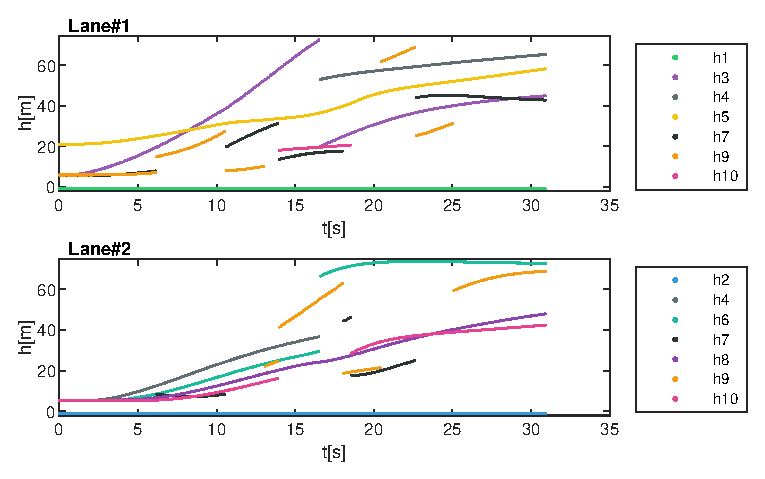
\includegraphics[width=0.8\textwidth]{eemobil/simh_case2}
			\caption{Red light traffic case 2. Headway of the vehicles respect to their position in lanes}
			\label{fig:red_light_situationh2}
		\end{figure}
		\begin{figure}
			\centering
			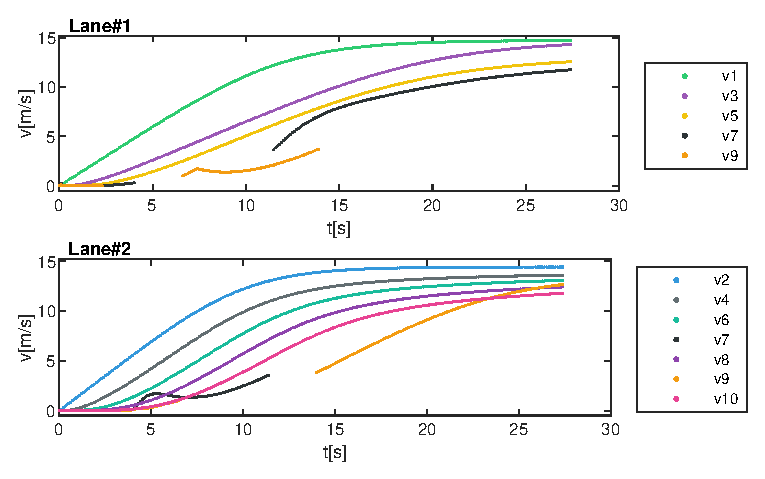
\includegraphics[width=0.8\textwidth]{eemobil/simv_case2}
			\caption{Red light traffic case 2. Velocity of the vehicles respect to their position in lanes}
			\label{fig:red_light_situationv2}
		\end{figure}
		\begin{figure}
			\centering
			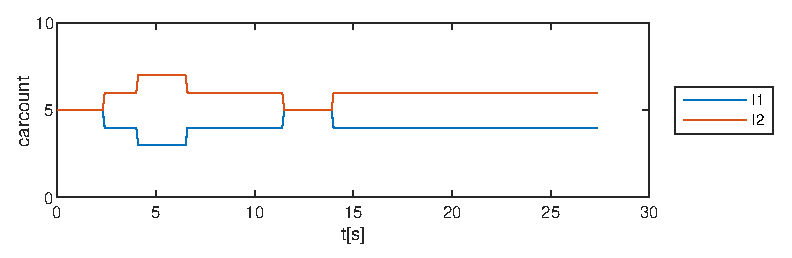
\includegraphics[width=0.8\textwidth]{eemobil/simcc_case2}
			\caption{Red light traffic case 2. Number of cars in lanes }
			\label{fig:red_light_situationcc2}
		\end{figure}
		\subsection*{Summary of the result}
		The results can be seen on Figure \ref{fig:red_light_situationh2}, \ref{fig:red_light_situationv2} and \ref{fig:red_light_situationcc2}.
		[TODO: Here comes the magnifier images.]

\end{document}
